\documentclass{article}%
\usepackage[T1]{fontenc}%
\usepackage[utf8]{inputenc}%
\usepackage{lmodern}%
\usepackage{textcomp}%
\usepackage{lastpage}%
\usepackage[head=40pt,margin=0.5in,bottom=0.6in]{geometry}%
\usepackage{graphicx}%
%
\title{\textbf{Familiares de Requesens rechazaron publicación de fotos del diputado}}%
\author{EFE}%
\date{05/10/2018}%
%
\begin{document}%
\normalsize%
\maketitle%
\textbf{URL: }%
http://www.el{-}nacional.com/noticias/politica/familiares{-}requesens{-}rechazaron{-}publicacion{-}fotos{-}del{-}diputado\_254568\newline%
%
\textbf{Periodico: }%
EN, %
ID: %
254568, %
Seccion: %
Política\newline%
%
\textbf{Palabras Claves: }%
Diputados, Política, Presos políticos, Gobierno\newline%
%
\textbf{Derecho: }%
1.2%
, Otros Derechos: %
5, 18%
, Sub Derechos: %
1.2.2%
\newline%
%
\textbf{EP: }%
NO\newline%
\newline%
%
\textbf{\textit{El padre del dirigente opositor afirmó desconocer el estado de salud de su hijo}}%
\newline%
\newline%
%
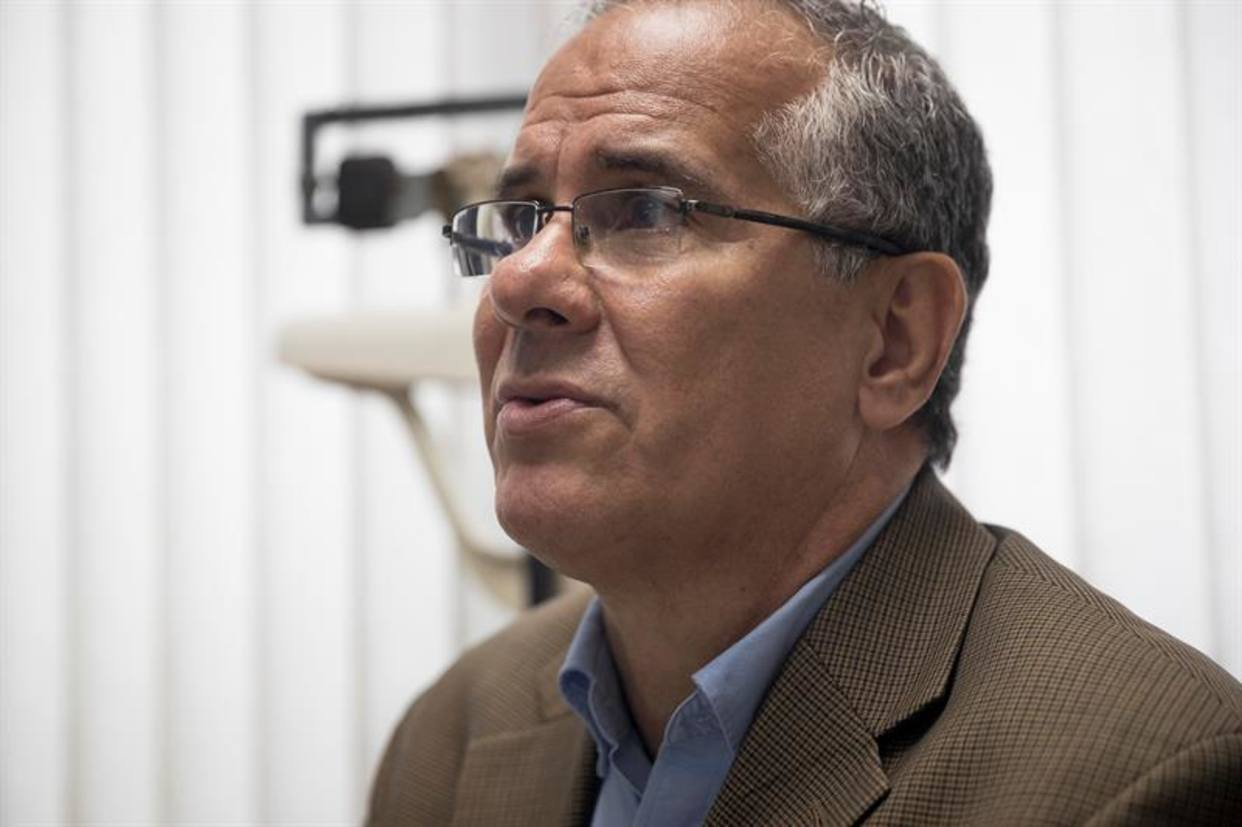
\includegraphics[width=300px]{164.jpg}%
\newline%
%
La familia de Juan Requesens,~diputado a la Asamblea Nacional, desmintió este viernes las pruebas presentadas por el gobierno venezolano en la Comisión Interamericana de Derechos Humanos (CIDH).%
\newline%
%
Juan Guillermo Requesens, padre del diputado, indicó a periodistas que al parlamentario se le están violando de manera sistemática sus derechos humanos pues, asegura, no tiene certeza de que se estén cumpliendo las indicaciones médicas en su caso.%
\newline%
%
"Mi preocupación es que esa foto que sacaron con unos médicos, si fue de ayer ¿Juan se sentía mal o no?, ¿tenía algún problema médico?, eso es un motivo de preocupación para mí como padre y médico y para toda la familia", afirmó.%
\newline%
%
Larry Devoe, secretario ejecutivo del Consejo Nacional de Derechos Humanos de Venezuela, aseguró este jueves ante la CIDH~que el gobierno venezolano garantiza los derechos de los privados de libertad.%
\newline%
%
Durante su exposición enseñó imágenes del~diputado~Requesens en las que se le puede apreciar caminando, durante “una visita familiar" y "recibiendo atención médica", según describió Devoe.%
\newline%
%
El hecho de que existan esas fotografías constituyen, según el padre de Requesens, otra violación a sus derechos debido a que el acto médico es confidencial, así como la visita de sus familiares deberían ser de carácter privado.%
\newline%
%
Juan Requesens fue~detenido~el 7 de agosto por funcionarios del Servicio Bolivariano de Inteligencia Nacional (Sebin) junto a su hermana Rafaela, quien fue puesta en libertad dos horas después, acusados de participar en el presunto intento de magnicidio registrado el 4 de agosto.%
\newline%
%
Tres días después de la detención del diputado, el gobierno difundió un video en el que se veía a Requesens, sentado frente a una cámara, “confesando” que formó parte en la organización del supuesto atentado, pero que actuó sin saber de qué se trataba, atendiendo a una solicitud del ex presidente de la Asamblea Nacional, Julio Borges.%
\newline%
%
También circuló un segundo video en el que se ve a Requesens en ropa interior aparentemente manchada de excrementos, sin pronunciar palabra.%
\newline%
%
Los familiares y el abogado de Requesens denunciaron que solo han podido ver al diputado en una ocasión luego de que fuera detenido.%
\newline%
%
\end{document}